%!TEX encoding = IsoLatin
%!TEX main = ../../main.tex

%\section{Self-Sovereign-Identity}
Self-Sovereign Identity (SSI) \cite{tobin2016inevitable} is a new model for digital identity. In the SSI ecosystem, a user can fully control his own identity and can use it between any service. SSI is different from today's digital identities: it is anchored to distributed ledgers so is not controlled by any centralized services.
One SSI innovation is the design and development of a common set of specifications: 
Decentralized Identifiers (DIDs) \cite{didW3C} and Verifiable Credentials (VCs) \cite{vcW3C}. 
Thanks to a standardised set of specifications, user identity can be anchored to different distributed ledgers, but it will also be defined in the same standard way.

\section{Decentralized Identifiers}  
DIDs \cite{didW3C} are identifiers referring to any subject determined by the controller of the DID.
A DID's controller can demonstrate control over a DID by design allowing a verifiable, decentralized digital identity, which will be independent of any identity providers, and certification authorities.

\subsection*{Overview}

A DID is a type of URI \cite{berners2005uniform} scheme that links a DID subject with a DID document allowing trustable interactions associated with that subject. The subject of a DID is the entity identified by the DID and can be a person, a group or an organization, a device, etc. Typically the DID subject is also the controller, but a DID can have more than one controller. 

Specifically, a DID is a simple text string, as shown in the figure \ref{didExample}, consisting of three parts: 
\begin{itemize}
    \item the DID URI scheme identifier
    \item the identifier for the DID method
    \item the DID method-specific identifier
\end{itemize}

\begin{figure}[h!]
    \centering
    \includesvg[inkscapelatex=false, scale=0.70]{./chapters/images/parts-of-a-did.svg}
    \caption{A simple example of a DID \cite{didW3C}.}
    \label{didExample}
\end{figure}

A DID document contains information about a DID subject and cryptographic material that will be used to prove control of that DID. DID documents can be represented in JSON \cite{json-rfc3986} or JSON-LD \cite{json-ld} format, as specified in W3C specification \cite{didW3C}. An example of DID document can be seen in Fig. \ref{didDocExample}. Only the controller of the DID has the right to make changes to the related DID document.

DIDs are generally stored in some underlying system or network for the resolution to DID documents. A verifiable data registry is a system that enables the recording of DIDs and the return of the data required to produce DID documents. Distributed ledgers, decentralized file systems, all types of databases, peer-to-peer networks, and other trusted data storage methods are some examples. The operations to create, resolve, update, and deactivate a DID and the related DID document are defined by DID methods and their specifications, which are generally coupled with a distinct verifiable data registry \cite{didW3C}. A DID \textit{resolves} to a DID document by using the \textit{read} operation of the applicable DID method \cite{didW3C}.
A DID URL expands the syntax of a DID with other standard components of URI such as path, query, and fragment to find a specific resource, such as a cryptographic public key inside a DID document or a resource outside the DID document. \\

% \begin{lstlisting}[caption={Example of a simple DID document from \cite{didW3C}.},captionpos=b,style=json, label={didDocExample},frame=single]
% {
%     "@context": [
%         "https://www.w3.org/ns/did/v1",
%         "https://w3id.org/security/suites/ed25519-2020/v1"
%     ]
%     "id": "did:example:123456789abcdefghi",
%     "authentication": [{

%         "id": "did:example:123456789abcdefghi#keys-1",
%         "type": "Ed25519VerificationKey2020",
%         "controller": "did:example:123456789abcdefghi",
%         "publicKeyMultibase": "zH3C2AVvLMv6gmMNam3uVAjZpfkcJCwDwnZn6z3wXmqPV"
%     }]
% }
% \end{lstlisting}

\begin{figure}[h!]
\begin{lstlisting}[style=json,frame=single]
{
    "@context": [
        "https://www.w3.org/ns/did/v1",
        "https://w3id.org/security/suites/ed25519-2020/v1"
    ]
    "id": "did:example:123456789abcdefghi",
    "authentication": [{

        "id": "did:example:123456789abcdefghi#keys-1",
        "type": "Ed25519VerificationKey2020",
        "controller": "did:example:123456789abcdefghi",
        "publicKeyMultibase": "zH3C2AVvLMv6gmMNam3uVAjZpfkcJCwDwnZn6z3wXmqPV"
    }]
}
\end{lstlisting}
\caption{Example of a simple DID document from \cite{didW3C}. \label{didDocExample}}
\end{figure}

\begin{figure}[h!]
    \centering
    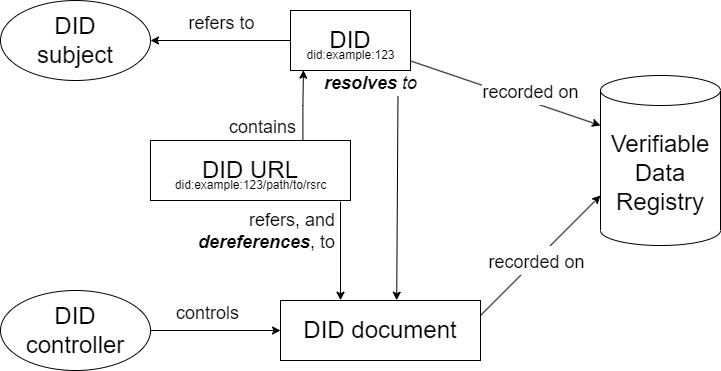
\includegraphics[width=12cm]{./chapters/images/did-overview.png}
    \caption{DID architecture overview and relationships between components \cite{didW3C}.}
    \label{didOverview}
\end{figure}

\section{Verifiable Credentials}
Verifiable Credential \cite{vcW3C} provides a standard method to express credentials on the internet in a way that is cryptographically safe, privacy-respecting, and machine-verifiable.
Outside the technological domain, a credential could consist of:
\begin{itemize}
    \item information related to identifying the subject of the credential (for example, a photo, name, or identification number)
    \item information related to the issuing authority (for example, a city government or a university)
    \item information related to the type of credential this is (for example, a passport or a driving license)
    \item information related to specific attributes or properties being asserted by the issuing authority about the subject (for example, nationality, the classes of vehicle entitled to drive, or date of birth)
    \item information related to constraints on the credential (such as expiration date, or terms of use). 
\end{itemize}

In verifiable credentials, the additional inclusion of digital signatures makes them more trustworthy and more tamper-evident compared to physical credentials. These allow third-party verified machine-readable personal information usable on the Web for receiving services and benefits as in the physical world \cite{vcW3C}.

\subsection*{Overview}

Distinct actors can be identified in the verifiable credentials ecosystem, which defines the roles and the relationships between them. The separation of roles allows the standardization of interfaces and protocols. In detail the existing entities that determine the so-called \textit{trust triangle} \cite{trustOverIP} are: 

\begin{itemize}
    \item \textit{holder}: his role is to request, possess or use verifiable credentials. Example holders include students, employees, and customers.
    \item \textit{issuer}: his role is to create a verifiable credential and provide that to a holder by asserting claims about one or more subjects. For example, an issuer is a government. 
    \item \textit{verifier}: his role is to process verifiable credentials provided by holders. Example verifiers are whoever provides a service. 
\end{itemize}

\begin{figure}[h!]
    \centering
    \includesvg[inkscapelatex=false, scale=0.70]{./chapters/images/vc-ecosystem.svg}
    \caption{The roles and information flows of Verifiable Credential \cite{vcW3C}.}
    \label{vcEcosystem}
\end{figure}

To use verifiable credentials with a specific verifier, a holder has to generate verifiable presentations.
A verifiable presentation encloses one or more verifiable credentials, issued by one or more issuers. Before presenting the verifiable presentation to a verifier, a holder signs the verifiable presentation content, proving authorship of the data and possession of verifiable credentials. 
However, The fact that a credential is verifiable by the verifier does not mean that the claims it contains are true. Another aspect that verifiable credentials enhance is privacy. 
The usage of machine-readable credentials allows malicious actors to collect and correlate data, compromising holders' privacy. 
Verifiable credentials specification draft how to deal with these issues, by using privacy-enhancing technologies, such as \textit{zero-knowledge proof} \cite{zkp-survey}. 

\begin{figure}[h!]
    \centering
    \includesvg[inkscapelatex=false, scale=0.45]{./chapters/images/credential.svg} 
    \hfil
    \includesvg[inkscapelatex=false, scale=0.45]{./chapters/images/presentation.svg}
    \caption{Basic components of a verifiable credential and a verifiable presentation \cite{vcW3C}.}
    \label{vc-vp-topview}
\end{figure}

Verifiable credentials and verifiable presentations can be represented in JSON \cite{json-rfc3986} or JSON-LD \cite{json-ld} format, as specified in W3C specification \cite{vcW3C}. Examples can be seen in \autoref{vcExample} and \autoref{vpExample}. \\

\begin{figure}[h!]
\begin{lstlisting}[style=json, breaklines=true,frame=single]
{   "@context": ["https://www.w3.org/2018/credentials/v1"],
    "id": "http://example.edu/credentials/1872",
    "type": ["VerifiableCredential", "AlumniCredential"],
    "issuer": "https://example.edu/issuers/565049",
    "issuanceDate": "2010-01-01T19:23:24Z",
    "credentialSubject": {
        "id": "did:example:ebfeb1f712ebc6f1c276e12ec21",
        "alumniOf": {
            "id": "did:example:c276e12ec21ebfeb1f712ebc6f1",
            "name": [{
                "value": "Example University",
                "lang": "en"
            }]
        }
    },    
    "proof": {
        "type": "RsaSignature2018",
        "created": "2017-06-18T21:19:10Z",
        "proofPurpose": "assertionMethod",
        "verificationMethod": "https://example.edu/issuers/565049#key-1",
        "proofValue": "eyJhbGciOiJSUzI1NiIsImI2NCI6ZmFsc2UsI..."
    }
}
\end{lstlisting}
\caption{A simple example of a verifiable credential \cite{vcW3C}. \label{vcExample}}
\end{figure}

% \begin{lstlisting}[caption={A simple example of a verifiable presentation \cite{vcW3C}.},captionpos=b,style=json, label={vpExample},breaklines=true,frame=single]
%     {
%         "@context": [
%           "https://www.w3.org/2018/credentials/v1",
%           "https://www.w3.org/2018/credentials/examples/v1"
%         ],
%         "type": "VerifiablePresentation",
%         "verifiableCredential": [{
%             ...
%         }],
%         "proof": {
%           "type": "RsaSignature2018",
%           "created": "2018-09-14T21:19:10Z",
%           "proofPurpose": "authentication",
%           "verificationMethod": "did:example:ebfeb1f712ebc6f1c276e12ec21#keys-1",
%           "challenge": "1f44d55f-f161-4938-a659-f8026467f126",
%           "domain": "4jt78h47fh47",
%           "proofValue": "Qy72IFLN25DYuNzVBAh4vGHSrQyHUGlc..."
%         }
%       }   
% \end{lstlisting}


\begin{figure}[h!]
\begin{lstlisting}[style=json, breaklines=true,frame=single]
{   "@context": ["https://www.w3.org/2018/credentials/v1"],
    "type": "VerifiablePresentation",
    "verifiableCredential": [{
        ...
    }],
    "proof": {
        "type": "RsaSignature2018",
        "created": "2018-09-14T21:19:10Z",
        "proofPurpose": "authentication",
        "verificationMethod": "did:example:ebfeb1f712ebc6f1c276e12ec21#keys-1",
        "challenge": "1f44d55f-f161-4938-a659-f8026467f126",
        "domain": "4jt78h47fh47",
        "proofValue": "Qy72IFLN25DYuNzVBAh4vGHSrQyHUGlc..."
    }
}   
\end{lstlisting}
\caption{A simple example of a verifiable presentation \cite{vcW3C}. \label{vpExample}}
\end{figure}
% \FloatBarrier   
\section{Distributed Ledgers Technologies}

Distributed Ledger Technology (DLT)  is a new paradigm for collecting and sharing information between people. A distributed ledger is a database that is spread across several nodes or computing devices in a network. An exact copy of the ledger is replicated and stored on each node. The revolutionary aspect of distributed ledger technology is that no single administrator or central authority is responsible for maintaining the ledger. Each network's participant node keeps its state updated by constructing and recording updates to the ledger independently. The nodes then vote on these adjustments to ensure that the majority agrees with the conclusion reached. This voting and agreement on the state of the ledger is called consensus and is conducted automatically via a consensus algorithm \cite{dlt-intro-1}. 
The following criteria can be used to categorize DLTs: data structures, consensus algorithms, permissions, mining accessibility and so on. The main data structure types are blockchains and Directed Acyclic Graphs (DAGs). Although blockchains are the most popular and well-known DLT type,  DLTs based on Directed Acyclic Graph (DAG) data structures are becoming more popular because they increase transaction speeds \cite{dlt-intro-2}. 
% reduce transaction data size and transaction fees, and
The key features of DLTs are:
\begin{itemize}
    \item decentralization: everyone can participate in consensus without being granted access. No single entity has control over the network
    \item immutability: the validated transaction cannot be altered. From a security point of view, this provides integrity to the data stored
    \item transparency: everyone can observe the transactions in the network
\end{itemize}

An Example of DAG DLT is \textit{The Tangle} of IOTA \cite{popov2018tangle}, a cryptocurrency for the IoT industry. IOTA offers the ability to transfer messages for free. There are several types of implemented messages. Some messages transfer value (the IOTA token or digital assets), while others transfer only pure data, and some message types can even contain both value and data. These properties make the Tangle suitable for storing SSI-related information. However, since the data on the Tangle are public, it may be necessary to protect them using encryption algorithms or other cryptographic protocols such as those described in \cite{iota-streams, ac1}.

\begin{figure}[h!]
    \centering 
    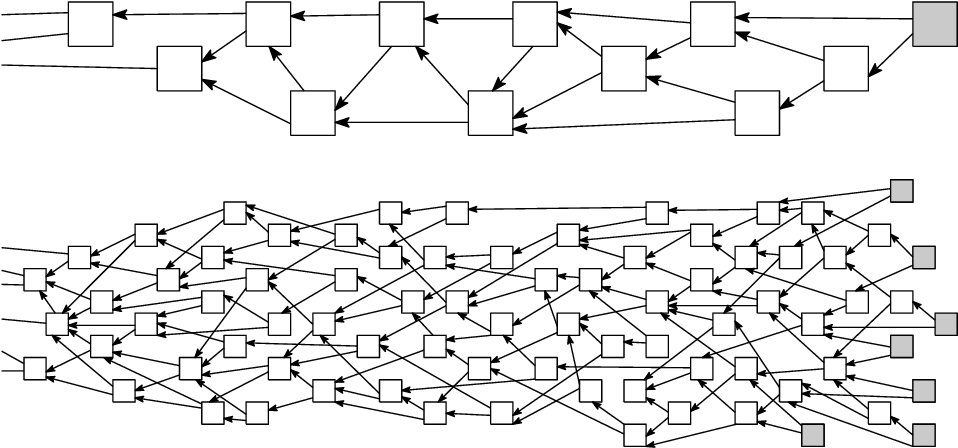
\includegraphics[width=10cm]{./chapters/images/tangle.png}
    \caption{Visualizations of the IOTA Tangle \cite{popov2018tangle}.}
    \label{tangleFigure}
\end{figure}

%parlare di come e' immutabile una blockchain?